\documentclass{standalone}
\usepackage{pgfplots}
\pgfplotsset{compat=1.11}
\begin{document}
% Place the TikZ picture in a figure environment.
%\begin{figure}[htb]
% h: here, t: top, b: bottom, p: page of float
%% https://tex.stackexchange.com/questions/39017/how-to-influence-the-position-of-float-environments-like-figure-and-table-in-lat
%% ! indicates that some restrictions should be ignored (discussed later)
%% h indicates that the float is allowed to be placed inline
%% t indicates that the float is allowed to go into a top area
%% b indicates that the float is allowed to go into a bottom area
%% p indicates the the float is allowed to go on a float page or column area

    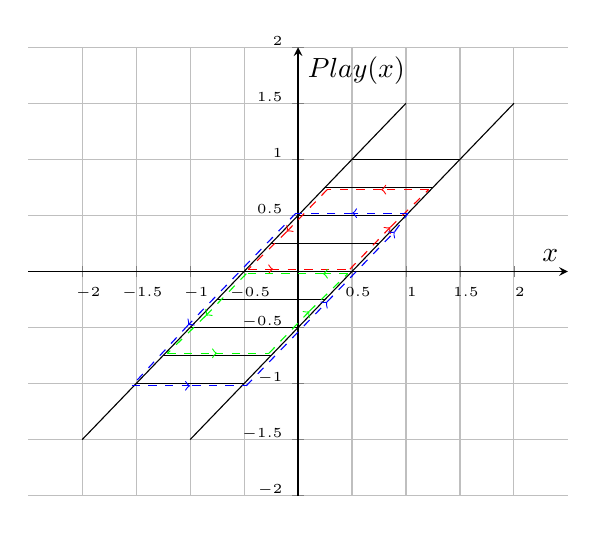
\begin{tikzpicture}
        \begin{axis} [
            xmin=-2.5, xmax=2.5, ymin=-2, ymax=2, grid=both,
            ylabel={$Play(x)$}, xlabel={$x$},
            xtick={-2,-1.5,...,2}, ytick={-2,-1.5,...,2},
            xticklabel style={font=\tiny, xshift=0.5ex},
            yticklabel style={font=\tiny, yshift=0.5ex},
            axis line style={->},
            axis x line=middle,
            axis y line=middle
        ]
        \addplot+[solid, mark=none, color=black, domain=-2:1] {x+0.5};
        \addplot+[solid,mark=none, color=black, domain=-1.5:-0.5] {-1};
        \addplot+[solid,mark=none, color=black, domain=-1.25:-0.25] {-0.75};
        \addplot+[solid,mark=none, color=black, domain=-1.0:0] {-0.5};
        \addplot+[solid,mark=none, color=black, domain=-0.75:0.25] {-0.25};
        \addplot+[solid,mark=none, color=black, domain=-0.5:0.5] {0};
        \addplot+[solid,mark=none, color=black, domain=-0.25:0.75] {0.25};
        \addplot+[solid,mark=none, color=black, domain=0:1] {0.5};
        \addplot+[solid,mark=none, color=black, domain=0.25:1.25] {0.75};
        \addplot+[solid,mark=none, color=black, domain=0.5:1.5] {1};
        
        \addplot+[solid,mark=none, color=black, domain=-1:2] {x-0.5};
        
        % red
        \addplot[dashed,->,color=red, thin] coordinates {(-0.5+0.04,0+0.02) (-0.25+0.02,0+0.02)};
        \addplot[dashed,-,color=red, thin] coordinates {(-0.25,0+0.02) (0.5-0.02,0+0.02)};
        \addplot[dashed,->,color=red, thin] coordinates {(0.5-0.02,0+0.02) (0.875-0.02,0.375+0.02)};
        \addplot[dashed,-,color=red, thin] coordinates {(0.875-0.02,0.375+0.02) (1.25-0.04,0.75-0.02)};
        \addplot[dashed,->,color=red, thin] coordinates {(1.25-0.04,0.75-0.02) (0.75+0.02,0.75-0.02)};
        \addplot[dashed,-,color=red, thin] coordinates {(0.75+0.02,0.75-0.02) (0.25+0.02,0.75-0.02)};
        \addplot[dashed,->,color=red, thin] coordinates {(0.25+0.02,0.75-0.02) (-0.125+0.02,0.375-0.02)};
        \addplot[dashed,-,color=red, thin] coordinates {(-0.125+0.02,0.375-0.02) (-0.5+0.04,0+0.02)};
        % green
        \addplot[dashed,->,color=green, thin] coordinates {(-1.25+0.04,-0.75+0.02) (-0.75,-0.75+0.02)};
        \addplot[dashed,-,color=green, thin] coordinates {(-0.75-0.02,-0.75+0.02) (-0.25-0.02,-0.75+0.02)};
        \addplot[dashed,->,color=green, thin] coordinates {(-0.25-0.02,-0.75+0.02) (0.125-0.02,-0.375+0.02)};
        \addplot[dashed,-,color=green, thin] coordinates {(0.125-0.02,-0.375+0.02) (0.5-0.04,0-0.02)};
        \addplot[dashed,->,color=green, thin] coordinates {(0.5-0.04,0-0.02) (0.25-0.02,0-0.02)};
        \addplot[dashed,-,color=green, thin] coordinates {(0.25-0.02,0-0.02) (-0.5-0.02,0-0.02)};
        \addplot[dashed,->,color=green, thin] coordinates {(-0.5+0.02,0-0.02) (-0.875+0.02,-0.375-0.02)};
        \addplot[dashed,-,color=green, thin] coordinates { (-0.875+0.02,-0.375-0.02) (-1.25+0.04,-0.75+0.02)};
        % blue
        \addplot[dashed,->,color=blue, thin] coordinates {(0.25+0.02,-0.25-0.02) (0.875+0.02,0.375-0.02)};
        \addplot[dashed,-,color=blue, thin] coordinates {(0.875+0.02,0.375-0.02) (1.+0.02,0.5+0.02)};
        \addplot[dashed,->,color=blue, thin] coordinates {(1.+0.02,0.5+0.02) (0.5,0.5+0.02)};
        \addplot[dashed,-,color=blue, thin] coordinates {(0.5,0.5+0.02) (0.-0.02,0.5+0.02)};
        \addplot[dashed,->,color=blue, thin] coordinates {(0.-0.02,0.5+0.02) (-1-0.02,-0.5+0.02)};
        \addplot[dashed,-,color=blue, thin] coordinates {(-1-0.02,-0.5+0.02) (-1.5-0.04,-1-0.02)};
        \addplot[dashed,->,color=blue, thin] coordinates {(-1.5-0.04,-1-0.02) (-1,-1-0.02)};
        \addplot[dashed,-,color=blue, thin] coordinates {(-1+0.02,-1-0.02) (-0.5+0.02,-1-0.02)};
        \addplot[dashed,->,color=blue, thin] coordinates {(-0.5+0.02,-1-0.02) (0.25+0.02,-0.25-0.02)};


        \end{axis}
    \end{tikzpicture}

\end{document}